%%%%%%%%%%%%%%%%%%% author.tex %%%%%%%%%%%%%%%%%%%%%%%%%%%%%%%%%%%
%
% sample root file for your "contribution" to a contributed volume
%
% Use this file as a template for your own input.
%
%%%%%%%%%%%%%%%% Springer %%%%%%%%%%%%%%%%%%%%%%%%%%%%%%%%%%


% RECOMMENDED %%%%%%%%%%%%%%%%%%%%%%%%%%%%%%%%%%%%%%%%%%%%%%%%%%%
\documentclass[graybox]{svmult}

% choose options for [] as required from the list
% in the Reference Guide

\usepackage{mathptmx}       % selects Times Roman as basic font
\usepackage{helvet}         % selects Helvetica as sans-serif font
\usepackage{courier}        % selects Courier as typewriter font
\usepackage{type1cm}        % activate if the above 3 fonts are
                            % not available on your system
%
\usepackage{makeidx}         % allows index generation
\usepackage{graphicx}        % standard LaTeX graphics tool
                             % when including figure files
\usepackage{multicol}        % used for the two-column index
\usepackage[bottom]{footmisc}% places footnotes at page bottom
% see the list of further useful packages
% in the Reference Guide
\usepackage{longtable}
\usepackage[utf8]{inputenc}
\usepackage{array}
\makeindex             % used for the subject index
                       % please use the style svind.ist with
                       % your makeindex program

%%%%%%%%%%%%%%%%%%%%%%%%%%%%%%%%%%%%%%%%%%%%%%%%%%%%%%%%%%%%%%%%%%%%%%%%%%%%%%%%%%%%%%%%%
\newcolumntype{C}[1]{>{\centering\let\newline\\\arraybackslash}m{#1}}

\begin{document}

\title*{Time-Series Price Prediction for Opportunistic Cloud Computing Resources}
\author{Sarah Alkharif , Kyungyong Lee, and Hyeokman Kim}
\institute{Sarah Alkharif \at Kookmin University, Seoul. South Korea, \email{saraalkharif@kookmin.ac.kr}
\and Kyungyong Lee \at Kookmin University, Seoul. South Korea, \email{leeky@kookmin.ac.kr}
\and Hyeokman Kim  \at Kookmin University, Seoul. South Korea, \email{hmkim@kookmin.ac.kr}
}
%
% Use the package "url.sty" to avoid
% problems with special characters
% used in your e-mail or web address
%
\maketitle

\abstract{Cloud computing resources are offered in various forms, and surplus of computing resources are provided at cheaper price. A leading cloud computing vendor, Amazon Web Services, provides such opportunistic resources as EC2 spot instance whose price changes dynamically based on the resource demand from users. We analyze the spot instance price logs and apply various predictive analysis algorithms to better predict future spot instance price. By applying various train dataset modeling heuristics, we uncover that the SARIMA algorithm achieves the best prediction accuracy in spot price prediction; it shows 17\% more accuracy than other algorithms that are widely used for spot instance applications. By applying contributions in this paper, we expect that spot instance users can decrease monetary cost while improving system stability.}

\section{Introduction}\label{sec:1}
Cloud computing provides various types of compute resources to serve diverse application scenarios. The cloud computing frees the burden of system administration overheads without incurring prohibitive initial hardware purchase cost. From the service provider's perspective, fully utilizing the already established hardware resources and services is crucial to maximize monetary gain. As the users' resource demand can vary from time to time, some cloud computing providers offer services at chaper price than the regular price to maximize hardware/service utilization. For instance, Amazon Web Services (AWS), a leading cloud computing vendor, provides its surplus of EC2 computing resources at a cheaper price in the form of \emph{spot instance}. A user who wants to use a spot instance bids for a price that one is willing to pay, and if the bid price is higher than the spot price that is decided by the service provider, one can get the resource allocated and pays for the spot price in the hourly basis. Other than AWS, Google Cloud Engine provides such opportunistic resources in the form of \emph{preemptive instances}, and Microsoft Azure provides its excess compute capacity as \emph{low-priority VM}.

Though users can utilize the opportunistic resources at a cheaper price, sudden service termination can happen at anytime as the demand for the computing resource changes. To mitigate the chance of sudden service interruption, few works were conducted to better predict and model the price change of EC2 spot instance in literature. Ben-Yehuda et al.~\cite{spot-instance-pricing-analysis} and Zhao et al.~\cite{spot-price-han-arima} tried to predict the future spot instance price using various predictive analysis algorithms, but they all concluded that the spot price is rather random and hard to make meaningful prediction for future price changes. Since then, most of studies that are related to spot instance focus on the handling sudden service interruption~\cite{tr-spark,spot-mpi-checkpoint,flint,deep-spot-cloud} or spot instance bid strategy~\cite{not-bid-cloud,how-to-bid-cloud}. 

In this paper, we apply various time-series analysis algorithms to predict price change pattern of AWS EC2 spot instances. By carefully desiging the period of train datasets, we could uncover that applying seasonal-arima (SARIMA) can improve the accuracy of price change prediction error by 17\% on average comparing to the naive method that references the most recent price to predict future price~\cite{deep-spot-cloud}. In addition to the contribution of improved price prediction accuracy, we could also discover that the configuration values to get the best prediction accuracy differs significantly across different availability zones and instance types. Based on the extensive experiments and promising results, we bring up an opportunity of improving spot instance prediction accuracy that can result in significant cost gain for cloud computing users with increased system stability.

\section{Time-Series Analysis for AWS EC2 Spot Instance Price}
In this work, we use various time-series analysis algorithms to predict future spot instince price. First, we apply a simple \emph{mean} method that uses the average of previous price to make prediction. In the \emph{mean} method, assuming the price of instance in time $t-1$ is $x_{t-1}$, to predict the price of an instance at time $t$, we use previous instance price until lag that is notated as $n$ (Equation~\ref{eq:mean}).

\begin{equation}
  \hat{y_{t}} = \frac{x_{t-1} +x_{t-2}+.....+x_{t-n}}{n}
\label{eq:mean}
\end{equation} 

Naive method is another simple model that references only the most recent spot instance price to make prediction for future time windows~\ref{eq:naive}. For naive and mean methods, the expected value can be used to make prediction for longer period of time later than $t$. 
\begin{equation}
  \hat{y_{t}} = x_{t-1} 
\label{eq:naive}
\end{equation}

Seasonal naive method is similar to naive method that uses the most recent observation, but it utilizes seasonal information in making prediction. Assuming the seasonal period is $s$, the predicted value at time $t$ is the observed value at time $t-s$~\cite{time-series-analysis}.
\begin{equation}
  \hat{y_{t}} = x_{t-s} 
\label{smean}
\end{equation}

Auto Regressive Integrated Moving Average (ARIMA) is a popular statistical model and widely applied for time series datasets. The algorithm is a combination of auto-regressive (Equation~\ref{Eq-AR}) and moving-average model (Equation~\ref{Eq-MA}), with three parameters  \((p,d,q)\). \(p\) is the number of auto-regressive terms that indicates dependencies on past values, \(d\) is the degree of differencing to make input dataset stationary, and \(q\) is the number of lagged forecast errors in the prediction equation that depends only on random error terms.
\begin{equation}
\hat{y_t} = w_0 +\beta_1 y_{t-1}+ \beta_2 y_{t-2}+.....\beta_n y_{t-n}+\epsilon_t
\label{Eq-AR}
\end{equation}
\begin{equation}
\hat{y_t} = w_0 +\epsilon_t + \delta_1 \epsilon_{t-1}+  \delta_2 \epsilon_{t-2}+...+ \delta_n \epsilon_{t-n}
\label{Eq-MA}
\end{equation}

If we set \(d = n\), the equation becomes 
\begin{equation}
\hat{y_t} = w_0 +\beta_1 y_{t-1}+ \beta_2 y_{t-2}+.....\beta_n y_{t-n} +  \delta_1 \epsilon_{t-1}+  \delta_2 \epsilon_{t-2}+...+ \delta_n \epsilon_{t-n}
\label{Eq-ARIMA}
\end{equation}

The term \(\beta_i \) is the weight that is applied to prior values in the time series, \(\delta_i \) is auto-correlation coefficients at lags, and \(\epsilon_i \) is the residual error term.

\begin{figure}
\centering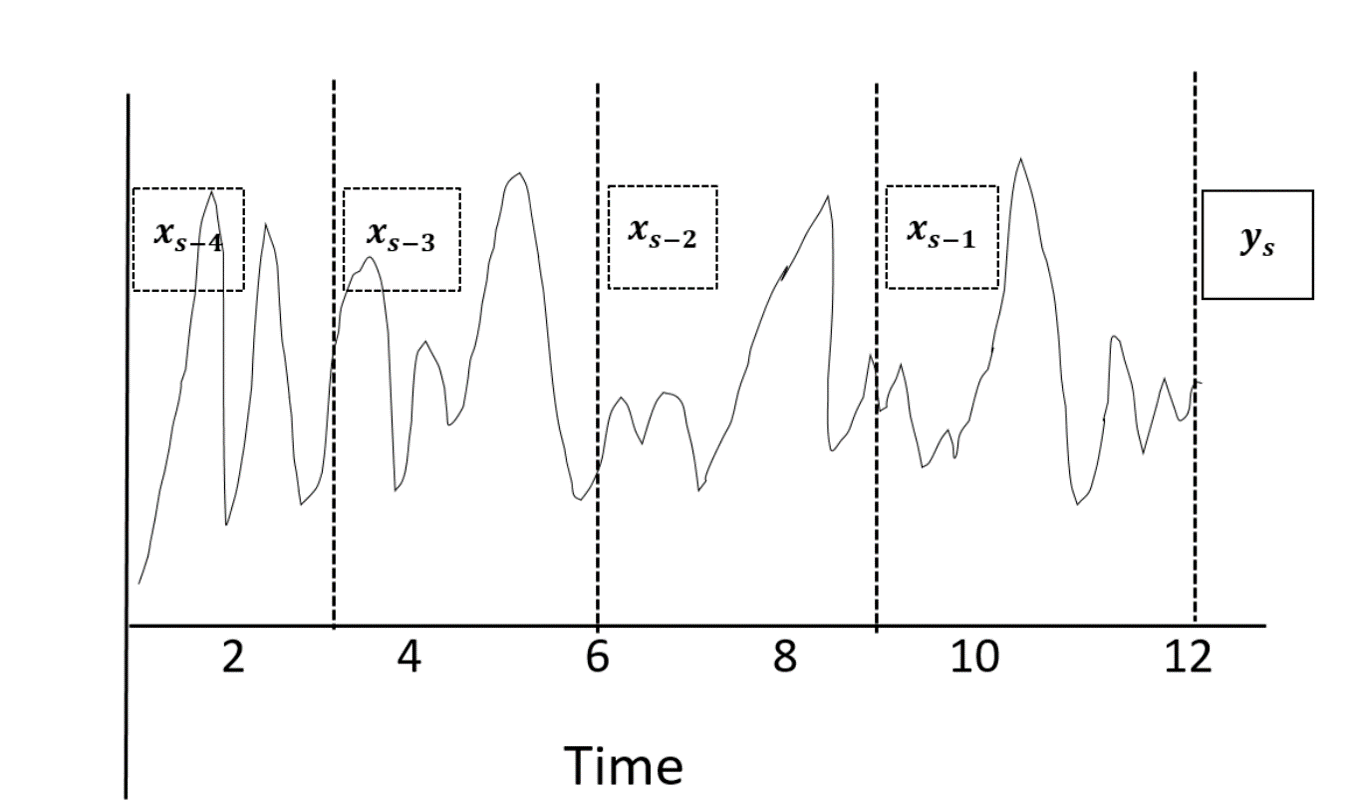
\includegraphics[width=0.7\textwidth]{figures/sarima.png}\caption{SARIMA example}\label{fig:sarima}
\end{figure}

SARIMA stands for Seasonal ARIMA that takes into account seasonal characteristics of input dataset, such as daily, monthly, or yearly. Figure~\ref{fig:sarima} shows an example dataset that is observed for one year and we will predict \(y_s\)  with seasonal  \(s= 4\) ,then the model will split length  of time series  to 4 quarterly seasonal periods for one year will be 3 months every period and then looking at same seasonal for all periods based on number of AR Eq.~\ref{Eq-AR} and MA Eq.~\ref{Eq-MA} then AR would be use \(\beta_{t-4}\) and MA  \(\delta_{t-4}\), second model MA would be  \(\beta_{t-4}\)  and \(\beta_{t-8}\) and AR \(\delta_{t-4}\) and \(\delta_{t-8}\).\\

Prophet model released by Facebook`s Core Data Science team ~\cite{prophet}, prophet model forecasting time series based on an additive model, non-linear model fit with seasonality and holidays like christmas ,it is required for historical datasets at least one year.
The prophet predect \(y_t\) by compute growth, seasonality and holidays:
\begin{equation}
\hat{y_t} = \beta_0 +\beta_1 y_{t-1}+ \beta_2 y_{t-2}+.....\beta_n y_{t-n}+\epsilon_t
\label{Eq-prophet}
\end{equation}
Where the term \(g_t\) is growth function to compute how the series has grown and the expected values for continue growing, and \(s_t\) seasonality change based on series behaviors ,\(h_t\) the effects of holidays ,\(\epsilon_t\) the error term.

\section{Evaluation}
To evalate the effectiveness of applying various algorithms to predict spot instance price, we fetch 11 months (from March. 2016 to Feb. 2017) of spot price log files from the AWS public API service. From the log files, we extracted the timestamp, spot price, availability zone, and instance type. As the on-demand instance price is different for different instance types in different regions, we normalize the spot instance price to that of on-demand instance. The normailized value indicates the cost gain that one can expect while using spot instances; smaller value indicates more gain.

At the time of writing, there are over 60s of AWS EC2 instance types that are served in over 30 availability zones. It becomes prohibitive to present the experiment results from all instance types, and we select representative instances in General, GPU, Compute-, Memory-, and Storage-optimized types that are m4.2xlarge, g2.2xlarge, c3.2xlarge, r3.2xlarge, and i2.2xlarge, respectively. The instances are not served in all availability zones, and we choose 18 zones that provide the aformentioned instance types for experiments.

We evaluate naive, seasonal naive, mean, seasonal ARIMA, linear regression, and Prophet algorithms using packages in R 3.2.4. Among them, linear regression and Prophet always perform worse than Arima, and we do not show the result from them. Different algorithms have distinct heuristics to choose the train dataset window. Naive and seasonal naive methods simply reference values from the previous observations. For mean method, we use previous 1, 3, 7, 15, 30, 60, 90, and 120 days of prices to get mean value for prediction. However, using only the most recent data (1 day) shows the best result, and we exclude other results. For seasonal Arima, we differentiate the training dataset period as 30, 60, 90, 120, and 150 days. In the prediction step, we use a model built by \textit{auto.arima} method of R. After building a model, we use the model for the next 1, 4, 8, 15, and 30 days. Overall, seasonal Arima has two configurations in the modeling data, \emph{previous days used in modeling, the number of days for a model to be used}, and we notate the value using parenthesis. For all algorithms, we predict the normalized spot instance price for the next 24 hours and calculate root-mean-squared-error to evaluate each model.

\begin{figure}
  \centering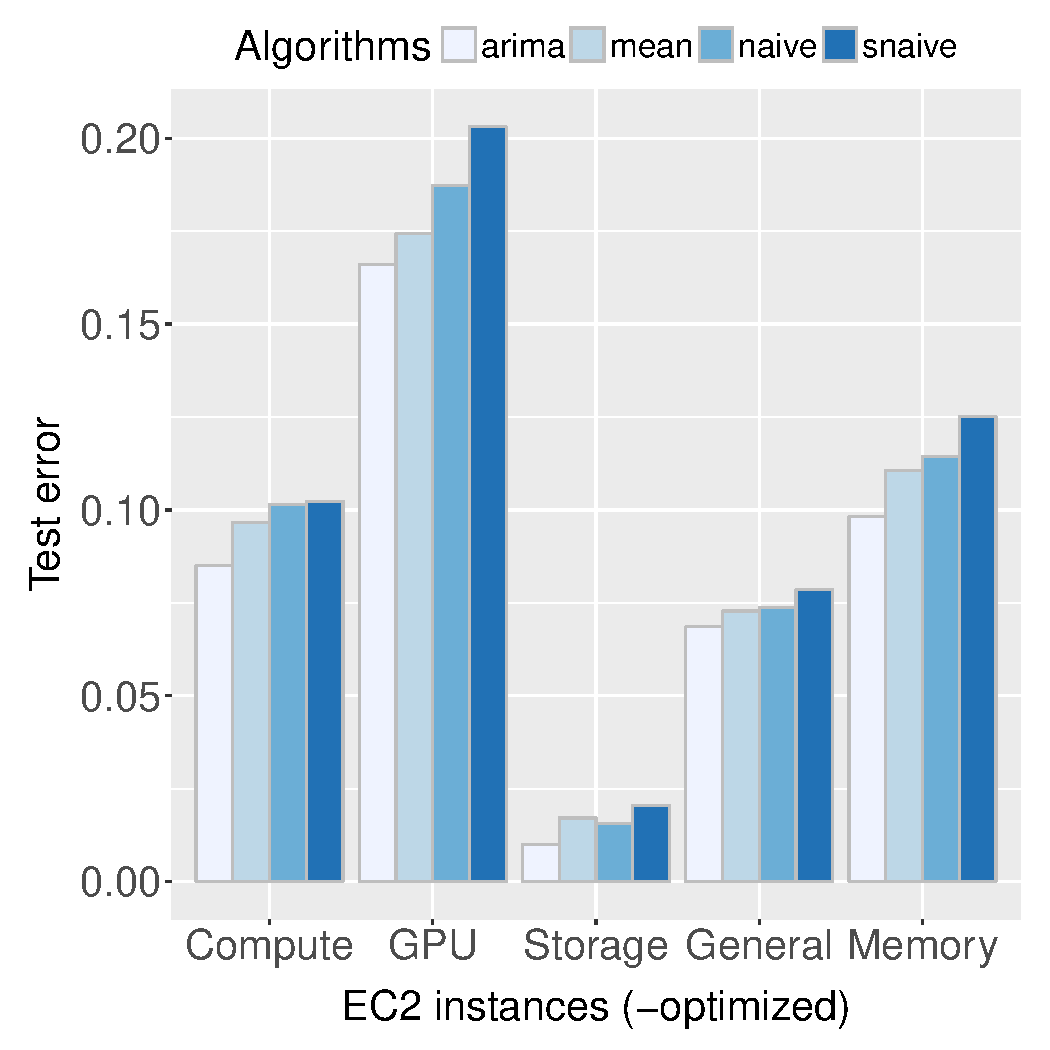
\includegraphics[width=0.7\textwidth]{figures/algorithm-compare-different-instance-type.pdf}\caption{Test error rates of different predictive algorithms. Regardless of the instance types, Arima shows the least error rate (lower is better).\label{fig:algo-diff-inst}}
\end{figure}

Figure~\ref{fig:algo-diff-inst} shows the test error of different algorithms. For seasonal Arima and mean, we select the best performing configuration values. Each algorithm is executed in all 18 availability zones, and the mean test error is presented. Regardless of instance types, Arima algorithm shows the best prediction accuracy among other methods. Previous works on predicting spot instance price insisted that using predictive analysis algorithms did not help to improve the prediction accuracy. With that, most systems using spot instances usually rely only on the very recent price (naive method) only. However, with thorough experiments and train data configuration, we could uncover the effectiveness of using Arima model to predict spot instance price for the first time. In the figure, we can observe that different instance types show different test error rate, and we expect the different hardware specifications, such as GPU cards, can result in distinct supply and demand pattern.  

\begin{figure}
  \centering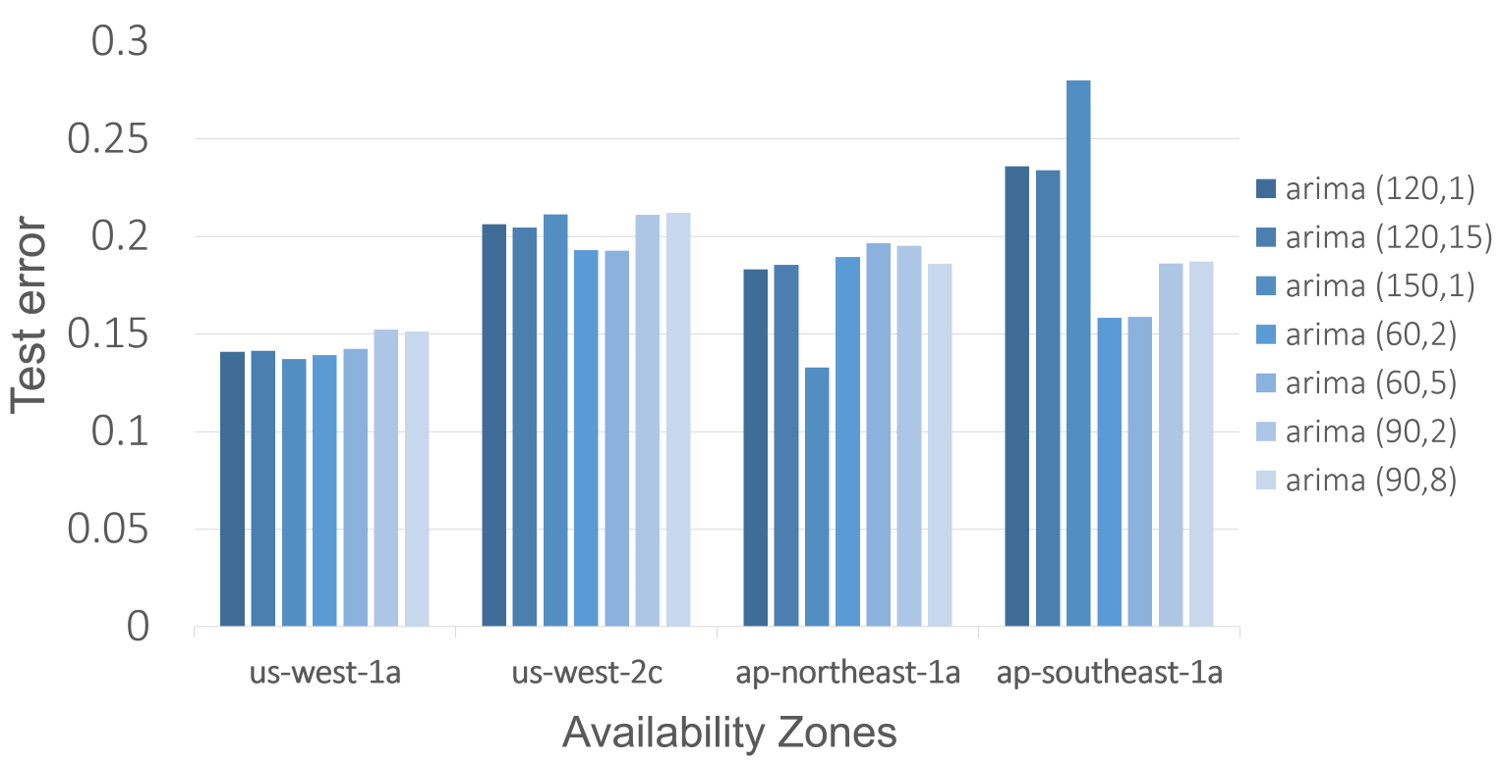
\includegraphics[width=1.2\textwidth]{figures/g2-4m-l.png}\caption{The impact of train data configurations to the overall test error rate of GPU instance (lower is better).\label{fig:g2-param-diverse}}
\end{figure}
From Figure~\ref{fig:algo-diff-inst}, we observed that the Arima algorithm shows the best performance. As noted earlier, we use various combinations of modeling data period and model use days. To see the effect from the different parameters, we show the test errors of GPU instances for different train data configurations in Figure~\ref{fig:g2-param-diverse}. The left two bars show the test error value of us-west-1a and us-west-2c that show the least impact from the distinct parameters. The right two bars show the test error of ap-northeast-1a and ap-southeast-1a that show the most impact from the paramters. Other availability zones that are not shown in the chart show the pattern in-beetween. In ap-southeast-1a zone, the worst configuration shows 50\% more error rate than the best configuration. Furthermore, the worst configuration in ap-southeast-1a (150, 1) is the best configuration for ap-northeast-1a. We suspect that such diversity was not considered in the previous works that try to predict spot instance price, and they could not eventually find a model to make better prediction. 
\begin{table}
  \begin{tabular}{ |C{2.5cm}||C{2cm}||C{2cm}||C{2cm}||C{2cm}|}
\hline
\small
\textbf{Availability Zones} &\textbf{General}&\textbf{Compute}&\textbf{Memory}&\textbf{Storage}\\\hline
ap-northeast-1a& (60,4)&(60,4)&(60,4)&(120,15)\\
ap-northeast-1c&(60,2)&(60,2)&(120,15)&(120,15)\\
ap-southeast-1a&(150,1)&(150,1)&(150,1)&(150,1)\\
ap-southeast-1b&(150,1)&(60,2)&(150,1)&(150,1)\\
ap-southeast-2a&(60,4)&(60,4)&(150,1)&(150,1)\\
ap-southeast-2b&(60,4)&(60,2)&(150,1)&(120,15)\\
eu-west-1a&(60,4)&(90,8)&(30,2)&(150,1)\\
eu-west-1b&(60,4)&(60,2)&(30,1)&(120,1)\\
eu-west-1c&(60,2)&(60,4)&(30,1)&(150,1)\\
us-east-1a&(50,1)&(150,1)&(30,1)&(60,2)\\
us-east-1c&(150,1)&(150,1)&(30,1)&(150,1)\\
us-east-1d&(60,2)&(150,1)&(30,2)&(150,1)\\
us-east-1e&(60,4)&(150,1)&(30,1)&(60,4)\\
us-west-1a&(60,2)&(150,1)&(30,1)&(120,15)\\
us-west-1b&(60,4)&(150,1)&(30,1)&(120,15)\\
us-west-2a&(60,2)&(150,1)&(150,1)&(150,1)\\
us-west-2b&(60,4)&(150,1)&(30,1)&(150,1)\\
us-west-2c&(60,2)&(60,2)&(60,2)&(150,1)\\\hline
\end{tabular}
\caption{Best Arima model configuration for different instance types in distinct availability zones}
\label{table:best-arima-config}
\end{table}

To check if there is optimal Arima train data configuration, we list the best performing train data parameters in Table~\ref{table:best-arima-config}. From the table, we can see that there is no globally optimal configurations. Contrary to general belief, building a model with train dataset with shorter time window sometimes performs better than longer train dataset. Furthermore, using a model longer period of time ocassionally perform better. From the table, we conclude that predicting spot instace price needs careful consideration in building train dataset, and the configuration needs to be dynamically updated. 


\section{Discussion and Future Work}
With thorough analysis about spot instance price prediction algorithms, we uncover the improved prediction accuracy as well as challenges in making better prediction. Based on the observation, we are going to further improve the algorithm in the following way.  

\textbf{The Good: Spot Price Change Prediction} Most of previous works that tried to predict spot instnace price concluded that the price is random, and applying predictive analysis algorithms does not really help to improve prediction quality~\cite{spot-instance-pricing-analysis,spot-price-han-arima}. In this work, we applied multiple time-series analysis algorithms by carefully designing the period of modeling data and parameters. With extensive evaluation, we could uncover that applying predictive analysis algorithms improves the price prediction accuracy over XY\% comparing to a method that uses only the most recent price~\cite{deep-spot-cloud,not-bid-cloud}.

\textbf{The Challenge: No Globally Optimal Model} Despite of increasing prediction accuracy by applying various techniques, we could not find the globally optimal algorithm and training data specification for different availability zones and distinct instance types. It makes challenging to apply the algorithms for real applications that can be deployed in any environments. 

\textbf{The Promising: Applying Hybrid Models} Even with the diversity of prediction accuracy for different algorithms and train data configuration, it is observed that the train error and test error show high correlation. Pearson product-moment correlation coefficient of train and test error is 0.904 - note that the coefficient has a value from -1.0 to 1.0, and the value of 1.0 means a perfect positive linear correlation, -1.0 means a negative correlation, while 0.0 means no correlation. We currently work on referencing the train error to better choose the algorithms and train data period. We are going to apply the heuristic to an application that utilizes GPU-based AWS EC2 spot instances to execute deep learning tasks in a cost efficient way~\cite{deep-spot-cloud}. 

\textbf{The Benefit: Lower Cost while Using Spot Instances} With the improvement in the prediction accuracy, we expect it will result in the cost gain by cherry-picking few availability zones and instance types with lower prices. We are working on a theoritical model that specifies correlation between the prediction accuracy and the real cost gain. We are also working to utilize the predicted outcome to anticipate instances that are likely to incur unexpected service interruption that is the crucial factor of making users reluctant to use spot instances. In the prediction step, we try to anticipate the spot instance price of the next 24 hours. In an ideal case, if the task migration cost among different availability zones and instane types are negligible, we can issue more frequent migrtations by relying on prediction module that has lower prediction error rate as the prediction window becomes shorter. By applying task migration heuristics that are proposed in literature~\cite{flint,deep-spot-cloud}, we expect to decrease the prediction time window to increase the accuracy.

\section{Related Work}
Since the introduction of spot instance from AWS EC2 service, many attempts were made to predict price change pattern in the near future.  
After thorough investigation of spot instance price logs, Ben-Yehuda et al.~\cite{spot-instance-pricing-analysis} concluded that applying predictive analysis algorithms in the prediction of spot instance price is meaningless as it changes randomly. Javadi et al.~\cite{availability-modeling} tries to apply statistical model to the price logs by applying MLE method. Though the approah helps to understand the spot price distribution, it does not help to predict future price. Similar to our work, Zhao et al.~\cite{spot-price-han-arima} applied ARIMA model to make spot instance price prediction, but they could not uncover the findings in this paper. The authors performed experiments only for one instance type in a single region. As shown in this paper, the price change pattern differs significant among different environments, and we expect the authors missed the characteristics.

As it was widely known that the spot instnace price is hard to be predicted, most recent work focused on increasing stability of applications that run on spot instances. DeepSpotCloud~\cite{deep-spot-cloud} and Flint~\cite{flint} proposed fast task migration mechanisms when a service interruption event happens. As the price prediction is challenging, both approaces used the naive method~\cite{how-to-bid-cloud,not-bid-cloud}, and we believe that the finding in this paper can significantly improve the cost gain and system stability of the previous approaches.

\section{Conclusion}
In this work, we try to predict future price for diverse instance types of AWS EC2 spot instances in 18 availability zones using various predictive analysis algorithms (naïve, seasonal naïve, mean, SARIMA, linear regression, Prophet) to see if they can help to better predict the future spot instance price. Different from what is generally known, we uncover that SARIMA model performs better than simple methods. To the authors' best knowledge, this is the first work that uncovers applying predictive analysis helps to better predict the future spot instance price. To get better result, we need to tune the train dataset by differentiating the modeling period and model use time, and the tuning steps needs to optimized to further improve the accuracy.  

\begin{acknowledgement}
This work is supported by the National Research Foundation of Korea (NRF) Grant funded by the Korean Government (MSIP) (No. NRF-2015R1A5A7037615 and NRF-2016R1C1B2015135), the ICT R\&D program of IITP (2017-0-00396), the AWS Cloud Credits for Research program.
\end{acknowledgement}
\bibliographystyle{spmpsci}
\bibliography{g2-price-modeling}
\end{document}
